\section{Tia Nur Candida (1174086)}
\subsection{Membaca Shapefile dengan PySHP}
\begin{enumerate}
	\item Nomor 1
	\lstinputlisting{src/tugas3/1174086/read1.py}
	\begin{figure}[H]
		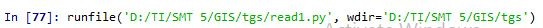
\includegraphics[width=6cm]{figures/Tugas3/1174086/No1.jpg}
		\centering
	\end{figure}
	\item Nomor 2
	\lstinputlisting{src/tugas3/1174086/read2.py}
	\begin{figure}[H]
		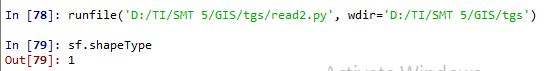
\includegraphics[width=6cm]{figures/Tugas3/1174086/No2.jpg}
		\centering
	\end{figure}
	\item Nomor 3
	\lstinputlisting{src/tugas3/1174086/read3.py}
	\begin{figure}[H]
		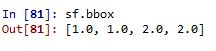
\includegraphics[width=6cm]{figures/Tugas3/1174086/No3.jpg}
		\centering
	\end{figure}
	\item Nomor 4
	\lstinputlisting{src/tugas3/1174086/read4.py}
	\begin{figure}[H]
		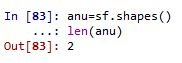
\includegraphics[width=6cm]{figures/Tugas3/1174086/No4.jpg}
		\centering
	\end{figure}
	\item Nomor 5
	\lstinputlisting{src/tugas3/1174086/read5.py}
	\begin{figure}[H]
		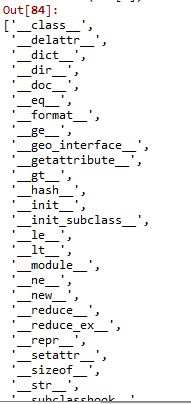
\includegraphics[width=6cm]{figures/Tugas3/1174086/No5.jpg}
		\centering
	\end{figure}
	\item Nomor 6
	\lstinputlisting{src/tugas3/1174086/read6.py}
	\begin{figure}[H]
		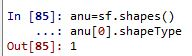
\includegraphics[width=6cm]{figures/Tugas3/1174086/No6.jpg}
		\centering
	\end{figure}
	\item Nomor 7
	\lstinputlisting{src/tugas3/1174086/read7.py}
	\begin{figure}[H]
		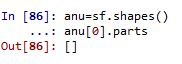
\includegraphics[width=6cm]{figures/Tugas3/1174086/No7.jpg}
		\centering
	\end{figure}
	\item Nomor 8
	\lstinputlisting{src/tugas3/1174086/read8.py}
	\begin{figure}[H]
		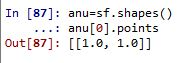
\includegraphics[width=6cm]{figures/Tugas3/1174086/No8.jpg}
		\centering
	\end{figure}
	\item Nomor 9
	\lstinputlisting{src/tugas3/1174086/read9.py}
	\begin{figure}[H]
		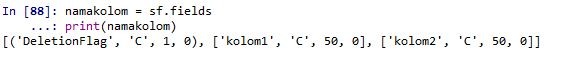
\includegraphics[width=6cm]{figures/Tugas3/1174086/No9.jpg}
		\centering
	\end{figure}
	\item Nomor 10
	\lstinputlisting{src/tugas3/1174086/read10.py}
	\begin{figure}[H]
		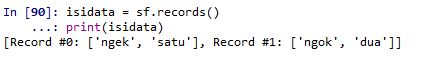
\includegraphics[width=6cm]{figures/Tugas3/1174086/No10.jpg}
		\centering
	\end{figure}
	\item Nomor 11
	\lstinputlisting{src/tugas3/1174086/read11.py}
	\begin{figure}[H]
		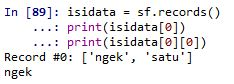
\includegraphics[width=6cm]{figures/Tugas3/1174086/No11.jpg}
		\centering
	\end{figure}
\end{enumerate}
\subsection{Link}
http://tiny.cc/sn0afz